

\chapter{为越南高等教育提出混合与适应性质量保障模型(V-AQA模型)}
\label{chap:de_xuat_vqa}

\section[引言]{引言:背景与新模型的紧迫性}
\addcontentsline{toc}{section}{引言}

基于第三章对越南高等教育质量保障体系现状及其系统性挑战的深入分析,得出了一个重要结论:现存问题之间存在因果联系,形成了复杂的“恶性循环”。世界银行的诊断报告已明确指出治理薄弱、培养与市场脱节以及质量保障体系尚未真正有效等问题\footcite{worldbank_improvingperformance}。这些问题并非孤立存在,而是相互交织,包括:大学自主权仍然有限\footcite{world-bank_improvingperformance},利益相关者参与度不高\footcite{pmc_article_9127449},质量文化带有浓厚的应付色彩\footcite{vjol_reactiveculture},以及质量保障人力资源既缺又弱\footcite{pmc_article_9127449}。

这表明,采用零散、片面的解决方案或机械地照搬国外的传统模式,将无法从根本上解决问题。越南需要一种新的方法,一个全面的行动框架,既能适应一个转型期经济体的特殊背景,又能与国际质量标准接轨。

为响应这一要求,本章将提出并详细论证一个新模型——\textbf{混合与适应性质量保障模型(简称V-AQA)}。该模型不仅是一系列孤立解决方案的集合,更是一个系统的思维和行动框架,旨在直接打破已指出的“恶性循环”,并从内部推动一种可持续的质量文化。

\section{越南现行质量保障框架的差距分析}
\label{sec:phan_tich_khoang_trong}

为申明V-AQA模型的紧迫性和适用性,首先需要分析在越南普遍应用的现有质量保障框架未能彻底解决的差距。

\subsection{东盟大学网络质量保障标准}

东盟大学网络及其质量保障标准在推动质量文化和区域一体化方面做出了巨大贡献。

\paragraph{优势} 东盟大学网络质量保障提供了一套全面的标准(4.0版共8项标准),重点关注成果导向教育和以学习者为中心\footcite{AUN-QAGuide}。获得东盟大学网络质量保障标准认证有助于越南的培养项目提升声誉,并为区域内的学生交换和学分互认创造便利条件\footcite{hoasen_benefits_aunqa}。

\paragraph{差距与局限}
\begin{itemize}
    \item \textbf{主要集中于课程层面:} 尽管有机构层面的标准,但在越南应用东盟大学网络质量保障标准主要发生在课程层面。这可能导致质量不均衡的状况,即少数几个项目达到国际标准,而整个机构,特别是在治理和资源分配方面,仍然沿用旧模式\footcite{aun_institutional_v2}。
    \item \textbf{流程复杂且成本高昂:} 寻求东盟大学网络质量保障认证需要大量的财政和人力资源,这为许多学校,特别是民办或地方院校设置了障碍\footcite{stdjssh_637}。
    \item \textbf{“形式化合规”的风险:} 获得认证的压力可能导致学校专注于完善档案和证据,以机械地满足标准,而不是从内部推动实质性改进\footcite{pmc_article_9127449}。
\end{itemize}

\subsection{教育培训部的规定}
教育培训部的法规文件体系,特别是关于质量认证的通知(如基于东盟大学网络质量保障标准制定的第12/2017号通知),为质量保障活动创造了强制性的法律走廊。

\paragraph{优势} 教育培训部的规定在整个体系内设立了最低质量要求,迫使教育机构进行自评和外部认证,有助于提升对质量保障的普遍认识。

\paragraph{差距与局限}
\begin{itemize}
    \item \textbf{体系缺乏独立性:} 各教育质量认证中心仍受教育培训部的直接管理,这引发了关于国家管理机构与专业认证机构之间客观性和独立性的担忧\footcite{ncdt_journal_219}。
    \item \textbf{大学自主权仍然有限:} 尽管自主政策已经颁布,但执行中仍存在诸多障碍。根据世界银行的报告,只有一小部分公立大学真正参与了自主试点,且自主范围仍然狭窄,特别是在组织和人事方面\footcite{world-bank_improvingperformance}。这降低了学校根据自身需求灵活改进质量的能力。
    \item \textbf{合规文化:} 按照教育培训部规定进行的认证通常被视为一项必须完成的行政义务,导致了“应付式合规”文化,而非内在的改进需求\footcite{vjol_reactiveculture}。
\end{itemize}

\subsection{构思-设计-实现-运作能力框架}
构思-设计-实现-运作是一个先进的框架,被越南许多工科院校采用,以改革培养方案,使其满足企业要求。

\paragraph{优势} 构思-设计-实现-运作提供了一个集成的学习框架,将理论与实践相结合,帮助学生全面发展个人、沟通和专业技能。应用构思-设计-实现-运作极大地推动了工科院校教学方法的创新\footcite{vietnamplus_cdio_reform}。

\paragraph{差距与局限}
\begin{itemize}
    \item \textbf{范围狭窄且难以推广:} 构思-设计-实现-运作主要为工程和技术学科设计。将该模型应用于社会科学、经济学或师范等学科是一个巨大挑战。
    \item \textbf{要求深刻的文化变革:} 成功实施构思-设计-实现-运作要求在思维和组织文化上发生重大变革,从领导层到每一位教师。在越南的研究已指出这种变革的困难,包括初期领导层缺乏正式承诺以及核心教师团队与其余人员之间互动有限\footcite{nguyen_cdio_2016}。
\end{itemize}

\section{V-AQA模型的定位:比较优势与优越性}
\label{sec:dinh_vi_vqa}

基于对上述差距的分析,提出V-AQA模型并非旨在完全替代,而是为了整合并克服现有框架在越南特殊背景下未能彻底解决的固有弱点。

与这些模型相比,V-AQA拥有突出的优势:
\begin{itemize}
    \item \textbf{混合性:} 主动平衡来自外部的\textbf{问责制}压力(教育培训部的要求)和来自内部的\textbf{持续改进}动力(东盟大学网络质量保障和构思-设计-实现-运作的精神),而不是只关注一个方面。
    \item \textbf{适应性:} 按照灵活的短期改进周期运作,帮助学校快速响应市场变化,而不是遵循僵化的长期计划。
    \item \textbf{全面性与内生性:} 作用于学校的全部五个核心方面(领导与治理、文化、利益相关者、流程、合作),并推动来自内部的变革(内生性),而不仅仅是遵守外部要求。
    \item \textbf{技术整合性:} 以管理信息系统为“神经系统”,使基于证据的治理成为可能,这是其他框架未直接提及的因素。
\end{itemize}

为更清晰地说明这种差异,下表将V-AQA与越南普遍应用的框架进行对比:

\begin{table}[h!]
\centering
\caption{V-AQA模型与普遍应用框架的对比表}
\label{tab:doi_sanh_vqa}
\begin{tabular}{|p{3cm}|p{3.5cm}|p{3.5cm}|p{3.5cm}|}
\hline
\textbf{比较标准} & \textbf{东盟大学网络质量保障(课程层面)} & \textbf{教育培训部规定(第12号通知)} & \textbf{V-AQA模型(建议)} \\
\hline
\textbf{主要目标} & 根据东盟共同标准评估、比对课程质量。 & 为各校规定最低标准和强制性认证流程。 & \textbf{从内部创建一个全面、自我改进且可持续的质量体系。} \\
\hline
\textbf{应用范围} & 主要在培养课程层面。 & 课程层面和教育机构层面。 & \textbf{全面覆盖学校层面,从领导、文化到每一个流程。} \\
\hline
\textbf{自主程度} & 学校自愿参加,但必须严格遵守东盟大学网络流程。 & 低,认证机构仍依赖教育培训部,合规性强\footcite{ncdt_journal_219}。 & \textbf{高且有导向:推动自主与通过关键绩效指标明确问责相结合。} \\
\hline
\textbf{利益相关者参与} & 有提及,但实际上学生和企业参与仍然有限\footcite{pmc_article_9127449}。 & 咨询性质,缺乏实质性约束机制。 & \textbf{将利益相关者的角色机制化(行业咨询委员会、学术委员会中的学生代表)。} \\
\hline
\textbf{灵活性} & 标准化流程,灵活性低。 & 规定具有普遍适用性,较为僵化。 & \textbf{高,是核心原则(适应性),允许根据短期周期进行调整。} \\
\hline
\end{tabular}
\end{table}

\textit{(注:构思-设计-实现-运作能力框架未直接纳入比较表,因为其本质是针对工科领域的专门培养方案开发框架,与东盟大学网络质量保障和教育培训部规定的综合性质量保障体系性质不同)。}

上表显示,V-AQA不仅是一套标准,更是一个\textbf{治理框架}。V-AQA不只关注“需要达成什么”,更关注“如何”构建一个能够自我改进的组织。这种方法直接解决了自主、质量文化和利益相关者参与等基础性问题,而仅仅应用单一标准是无法触及这些问题的。

为更深入地理解塑造这些比较优势的思想基础,下一部分将深入论证V-AQA模型的混合理念与适应性原则。


% het goi 1


\section{V-AQA模型的哲学基础与原则}
\label{sec:triet_ly_nguyen_tac_vqa}

V-AQA模型建立在两大哲学基础上,这两大基础是从国际研究和对越南特殊背景的分析中总结出来的:混合哲学与适应性原则。这正是该模型的“灵魂”,塑造了其所提出的方法和解决方案。

\subsection{混合哲学:协调问责制与质量改进}

越南高等教育体系目前正承受着双重压力。一方面,由于国家的主导作用和对公共预算的依赖,各大学必须强有力地满足\textbf{问责制}的要求。另一方面,在日益激烈的竞争和劳动力市场要求的背景下,各大学又迫切需要进行\textbf{改进}以提升质量和品牌。

这两个目标常常产生矛盾,导致要么过分注重形式上的合规以满足外部要求,要么是自发、无纪律的内部改进。V-AQA模型的“混合”哲学正是为了解决这种紧张关系而提出的。正如哈维和威廉姆斯(2010)在对高等教育质量十五年的综述中所分析的,一个有效的体系必须设法整合并协调这两个目标\footcite{harvey_williams_2010}。V-AQA模型通过承认外部透明的问责要求可以为推动内部改进努力提供必要的数据和压力来实现这一点。反之,强大的改进文化将使学校更容易满足并超越问责要求。这种方法有助于将关系从对抗转为共生,其中遵守规定成为前提,而提升质量成为最终目标。

\subsection{适应性原则:在变化背景下的灵活性}

越南的经济社会和政策背景正在以极快的速度变化。第四次工业革命、关于大学自主的新政策以及劳动力市场的波动,都要求质量保障体系必须具有高度的灵活性。一个为期五年的僵化质量改进计划,有可能在尚未执行完毕时就已经过时。

因此,V-AQA模型建立在“适应性”原则之上,其灵感来自于像适应性项目框架这样的敏捷项目管理框架\footcite{Wysocki2009}。该原则鼓励采用短期的、重复的改进周期,而不是一个长期的PDCA循环。各学校可以按学年甚至学期设定质量目标,实施、快速收集反馈数据,并为下一个周期调整计划。这种方法帮助各学校“边做边学”,最大限度地减少长期错误决策的风险,并确保改进努力始终与不断变化的实际背景相符。

\section{V-AQA模型的总体结构与要素}
\label{sec:cau_truc_tong_the}

基于上述两大哲学基础,V-AQA模型被建构为一个由理论基础、五个相互作用的核心要素和最终目标组成的总体结构。

\begin{figure}[h!]
    \centering
    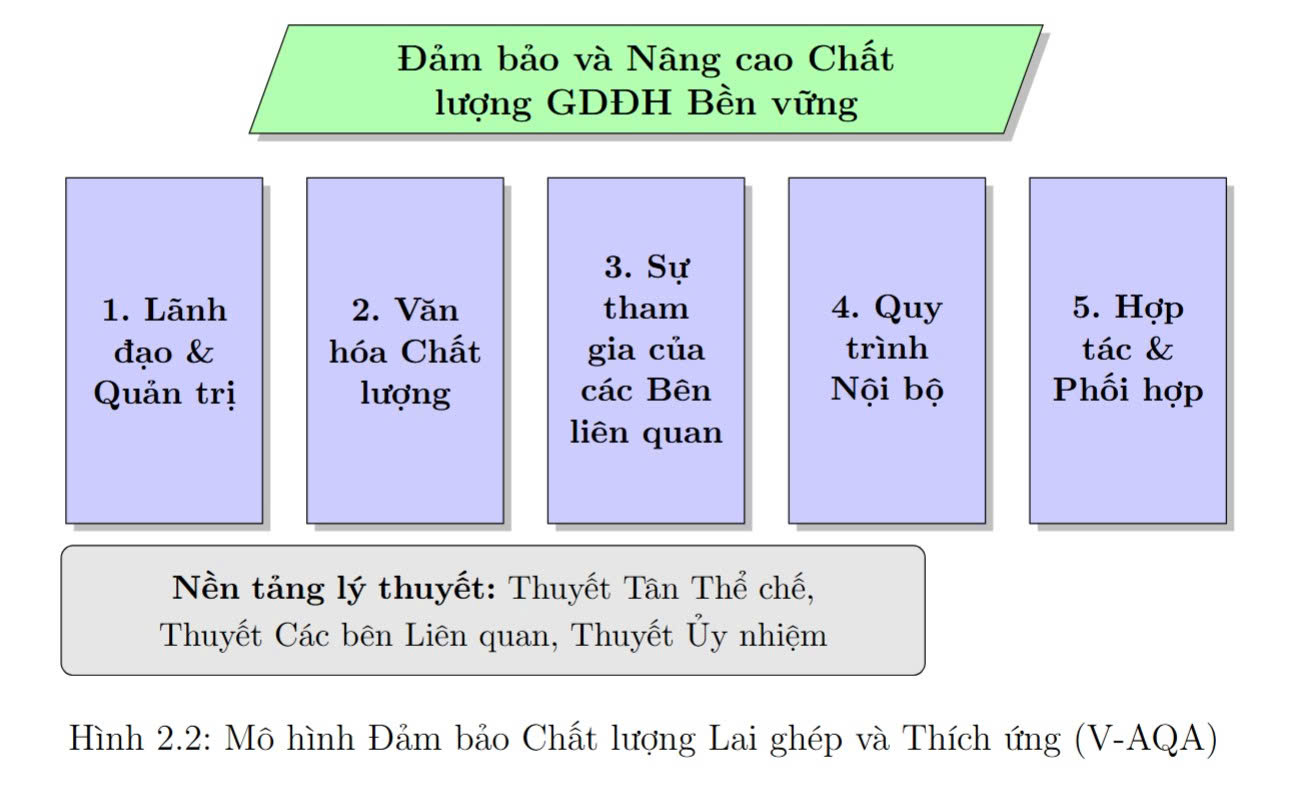
\includegraphics[width=\textwidth]{image/mo_hinh_V-AQA.jpg}
    \caption{混合与适应性质量保障模型 (V-AQA)}
    \label{fig:v-aqa-model-detailed}
\end{figure}

V-AQA模型的五个要素相互作用,形成一个完整的质量体系。为给读者,特别是那些非质量保障领域的专业人士,提供一个全面且易于理解的概览,下表将总结每个要素的目标、具体表现以及建议的关键绩效指标。该表如同一张“地图”,为后续的详细分析部分勾画了结构。

\begin{longtable}{|p{2.5cm}|p{3.5cm}|p{4.5cm}|p{3.5cm}|}
\caption{V-AQA模型5要素总结}
\label{tab:tong_hop_5_thanh_to}\\
\hline
\textbf{要素} & \textbf{主要目标} & \textbf{具体表现(行动)} & \textbf{衡量方式(关键绩效指标示例) \footcite{uq_kpi_dashboard}} \\
\hline
\endfirsthead
\multicolumn{4}{c}%
{{\bfseries \tablename\ \thetable{} -- 续前页}} \\
\hline
\textbf{要素} & \textbf{主要目标} & \textbf{具体表现(行动)} & \textbf{衡量方式(关键绩效指标示例) \footcite{uq_kpi_dashboard}} \\
\hline
\endhead
\hline \multicolumn{4}{r}{{续下页}} \\
\endfoot
\hline
\endlastfoot

% 第1行
\textbf{1. 领导与治理} & 将领导者从“控制者”转变为“环境创造者”。 & 
\begin{itemize}
    \item 制定并执行校级质量战略。
    \item 向院系下放强有力的权力并辅以问责制。
    \item 为中层管理团队提供能力提升培训。
\end{itemize} & 
\begin{itemize}
    \item 质量战略中各项目标的完成率。
    \item 各院系对自主权的满意度。
    \item 完成现代治理培训的中层管理者数量。
\end{itemize} \\
\hline

% 第2行
\textbf{2. 质量文化} & 从“应付式合规”文化转变为“主动改进”文化。 & 
\begin{itemize}
    \item 发起系统的质量宣传运动。
    \item 建立表彰和奖励改进创举的体系。
    \item 成立并授权“质量改进小组”。
\end{itemize} & 
\begin{itemize}
    \item 关于质量文化认知的定期调查得分。
    \item 每年提出并实施的改进创举数量。
    \item 参与改进活动的教职工比例。
\end{itemize} \\
\hline

% 第3行
\textbf{3. 利益相关者的参与} & 将利益相关者(企业、学生、校友)转变为“战略伙伴”。 & 
\begin{itemize}
    \item 将行业咨询委员会的活动机制化。
    \item 让学生代表在科学与培养委员会中拥有投票权。
    \item 建立主动的“校友大使”网络。
\end{itemize} & 
\begin{itemize}
    \item 行业咨询委员会的建议被整合到培养方案中的比例。
    \item 有学生代表参与的学术决策数量。
    \item 企业对毕业生契合度的满意度得分。
\end{itemize} \\
\hline

% 第4行
\textbf{4. 内部流程} & 基于数据实现学术和管理流程的现代化、标准化。 & 
\begin{itemize}
    \item 采用基于成果导向教育理念的培养方案开发流程。
    \item 多样化教学和评估方法。
    \item 构建并整合质量保障管理信息系统。
\end{itemize} & 
\begin{itemize}
    \item 按照成果导向教育流程制定和审查的培养方案比例。
    \item 课程中过程性评估分数的平均比重。
    \item 基于质量保障管理信息系统数据做出的管理决策比例。
\end{itemize} \\
\hline

% 第5行
\textbf{5. 合作与协调} & 打破“孤岛”状态和封闭思维,创造一个开放的质量生态系统。 & 
\begin{itemize}
    \item 为跨学科、跨单位的质量改进项目提供经费。
    \item 建立并参与标杆比对网络。
    \item 战略性地利用国际认证活动进行学习。
\end{itemize} & 
\begin{itemize}
    \item 成功实施的跨院系/部门项目数量。
    \item 组织的标杆比对活动及产生改进报告的数量。
    \item 国际认证建议的完成比例。
\end{itemize} \\
\end{longtable}

本章的后续部分将深入分析和论证上述五个要素中的每一个,包括建议的解决方案、科学依据、潜在风险及缓解策略。



% het goi 2 chuong 4




































